%----------------------------------------------------------------------------------------
%	PACKAGES AND THEMES
%----------------------------------------------------------------------------------------
\documentclass[aspectratio=169,xcolor=dvipsnames]{beamer}
\usetheme{Simple}

\usepackage{hyperref}
\usepackage{graphicx} % Allows including images
%\usepackage[export]{adjustbox} %throws error
\usepackage{booktabs} % Allows the use of \toprule, \midrule and \bottomrule in tables
\setbeamersize{text margin left=12mm, text margin right=12mm} 

\addtobeamertemplate{footline}{%
  \setlength\unitlength{1ex}%
  \begin{picture}(0,0) 
    % \put{} defines the position of the frame
    \put(134,83.6){\makebox(0,0)[bl]{
    
\includegraphics[scale=0.4]{images/uni_logo_weiss.eps}
    }}%
  \end{picture}%
}{}

\AtBeginSection[]{
  \begin{frame}
  \vfill
  \centering
  \begin{beamercolorbox}[sep=8pt,center,shadow=true,rounded=true]{title}
    \usebeamerfont{title}\insertsectionhead\par%
  \end{beamercolorbox}
  \vfill
  \end{frame}
}

%----------------------------------------------------------------------------------------
%	TITLE PAGE
%----------------------------------------------------------------------------------------

% The title
\title[Determination of political views]{Determination of political views}
\subtitle{using NLP on social media postings}

\author[Lennart Hallenberger, Florian Siepe]{Lennart Hallenberger, Florian Siepe}
\institute[] % Your institution may be shorthand to save space
{
    % Your institution for the title page
    Department Mathematics and Computer Science \\
    Philipps University of Marburg
    \vskip 3pt
}
\date{\today} % Date, can be changed to a custom date


%----------------------------------------------------------------------------------------
%	PRESENTATION SLIDES
%----------------------------------------------------------------------------------------

\begin{document}

\begin{frame}[plain]
    % Print the title page as the first slide
    \titlepage
    \begin{figure}[h]
        
\includegraphics[scale=0.5]{images/uni_logo_schwarz.eps}
    \end{figure}
\end{frame}

\begin{frame}{Outline}
    % Throughout your presentation, if you choose to use \section{} and \subsection{} commands, these will automatically be printed on this slide as an overview of your presentation
    \tableofcontents
\end{frame}

%------------------------------------------------
\section{Goal (revisited)}
%------------------------------------------------

\begin{frame}{Goal (revisited)}

    \begin{block}{Main objective}
        Classify social media postings to match them with a political party.
    \end{block}
    
    \begin{block}{Approach}
        \begin{itemize}
            \item Use posts from known politicians with their political party as label
            \item Data cleaning and pre-processing
            \item Use LDA to extract topics from postings (Topic Modeling)
            \item Train classifier, predict and evaluate
        \end{itemize}
    \end{block}
\end{frame}

%------------------------------------------------
\section{Overview of the dataset}
%------------------------------------------------

\begin{frame}{Overview of the dataset}
    \begin{block}{Democrat vs Republican Tweets}
        \begin{itemize}
            \item 84502 Tweets
            \item 433 Accounts
            \item 51\% Republican
            \item 49\% Democrat
            \item 200 last tweets from known members of Democratic and Republican party
            \item Collected from May 2018
        \end{itemize}
    \end{block}
\end{frame}

\begin{frame}{ML-Pipeline}
    \begin{figure}
        \centering
        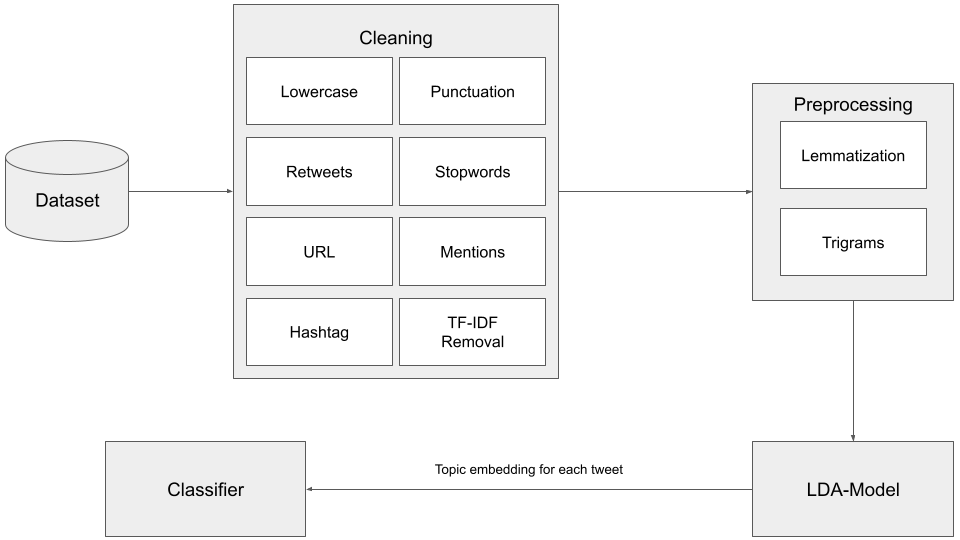
\includegraphics[width=.8\textwidth]{images/pipeline.png}
        \caption{ML-Pipeline}
        \label{fig:pipeline}
    \end{figure}
\end{frame}

%------------------------------------------------
\section{Benchmarks}
%------------------------------------------------

\begin{frame}{Perplexity}
    \vspace{-10mm}
    \begin{figure}
        \centering
        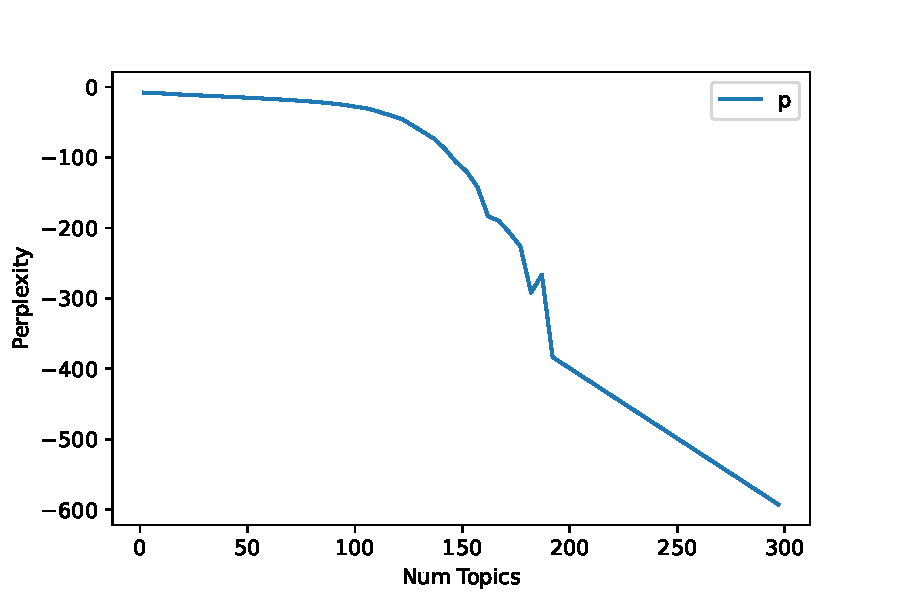
\includegraphics[width=.8\textwidth]{images/topic_count.pdf}
        \caption{Perpexlity over \# topics}
        \label{fig:perplexity}
    \end{figure}
\end{frame}

\begin{frame}{Distinction matrix}
    \vspace*{-5mm}
    \begin{columns}
        \hspace{-5mm}
        \begin{column}{.7\textwidth}
            \begin{figure}
                \centering
                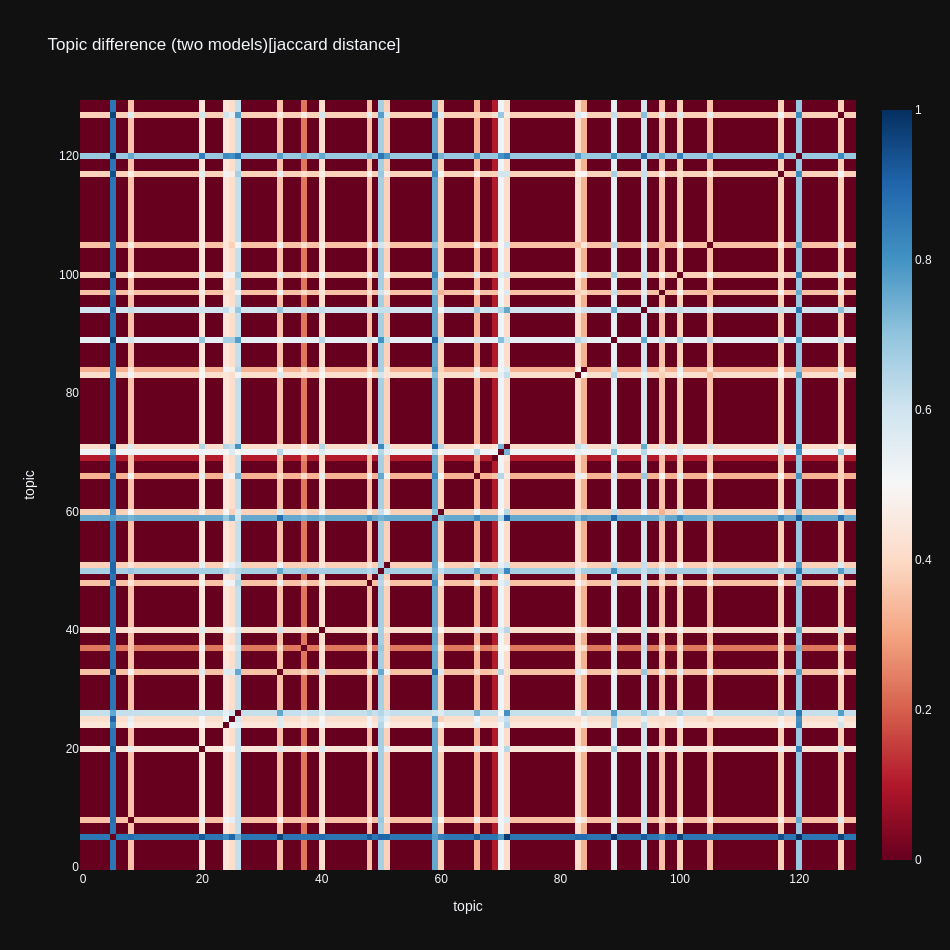
\includegraphics[width=.65\linewidth]{images/dem_dem_diff_130.png}
                \caption{130 Topics}
                \label{fig:dem_dem_diff_130}
            \end{figure}
        \end{column}
        \hspace*{-2cm}
       \begin{column}{.7\textwidth}
            \begin{figure}
                \centering
                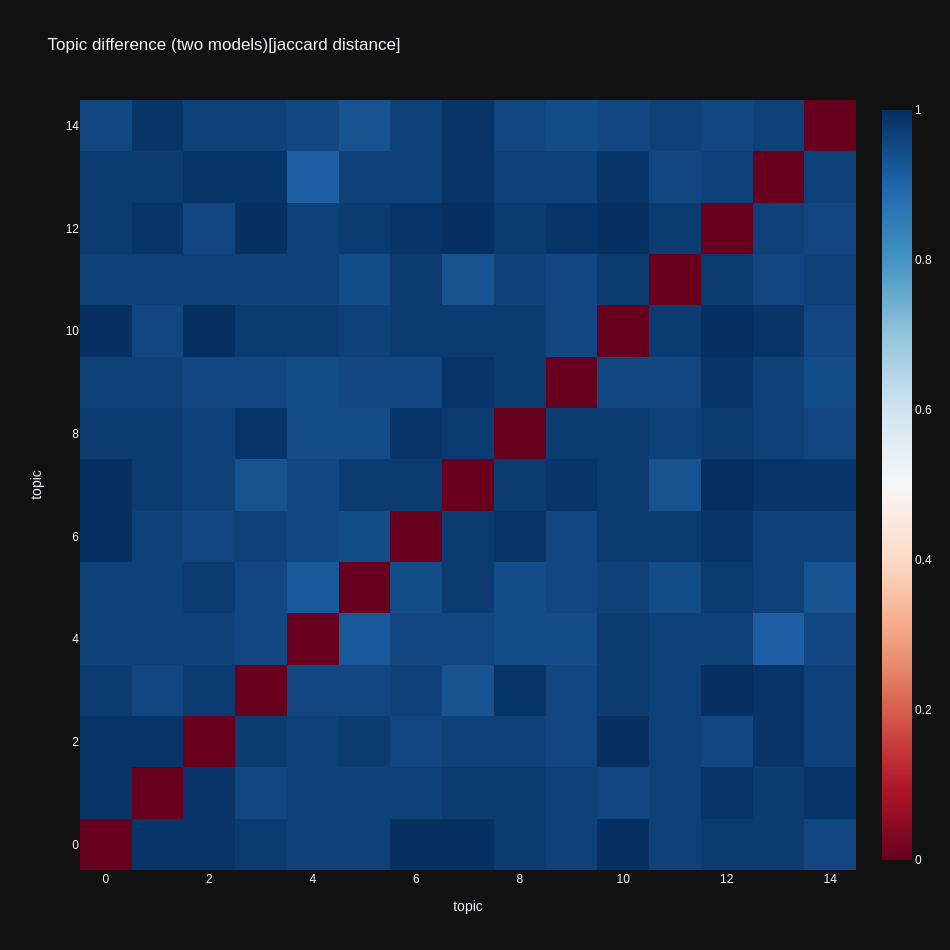
\includegraphics[width=.65\linewidth]{images/dem_dem_diff_15.png}
                \caption{15 Topics}
                \label{fig:dem_rep_diff_130}
            \end{figure}
        \end{column}
    \end{columns}
\end{frame}

\begin{frame}{Precision \& Recall}
    \vspace*{-10mm}
    \begin{columns}
        \hspace{-5mm}
        \begin{column}{.7\textwidth}
            \begin{figure}
                \centering
                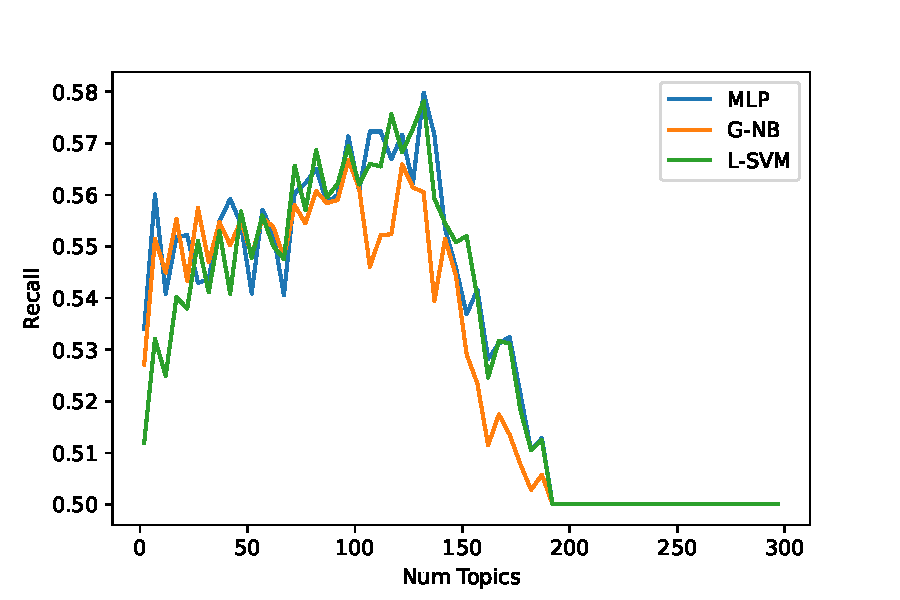
\includegraphics[width=.9\linewidth]{images/topic_recall.pdf}
                \caption{Recall over \# topics}
                \label{fig:rec}
            \end{figure}
        \end{column}
        \hspace*{-2cm}
       \begin{column}{.7\textwidth}
            \begin{figure}
                \centering
                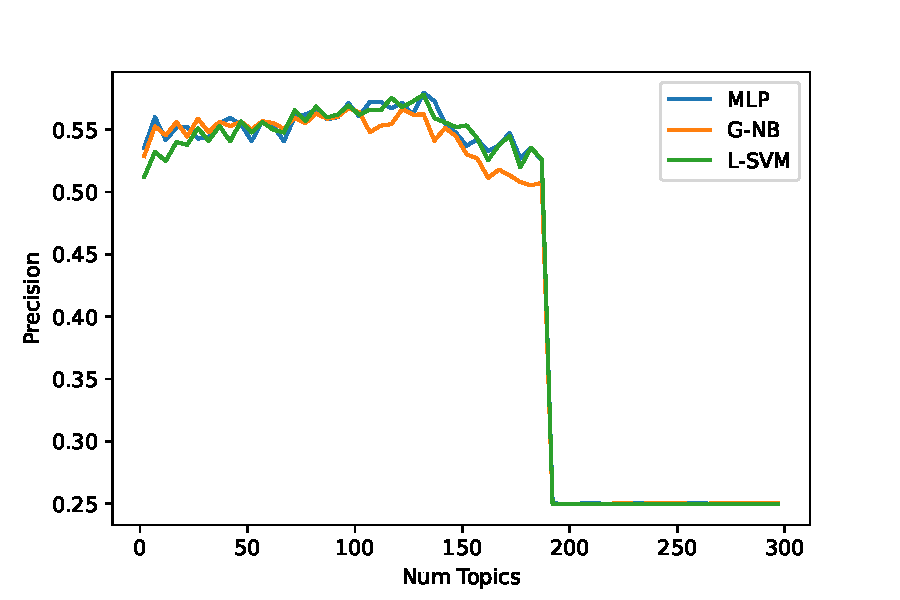
\includegraphics[width=.9\linewidth]{images/topic_precision.pdf}
                \caption{Precision over \# topics}
                \label{fig:pre}
            \end{figure}
        \end{column}
    \end{columns}
\end{frame}

\begin{frame}{Confusion \& F$_1$-Score}
    \vspace*{-10mm}
    \begin{columns}
        \hspace{-5mm}
        \begin{column}{.7\textwidth}
            \begin{figure}
                \centering
                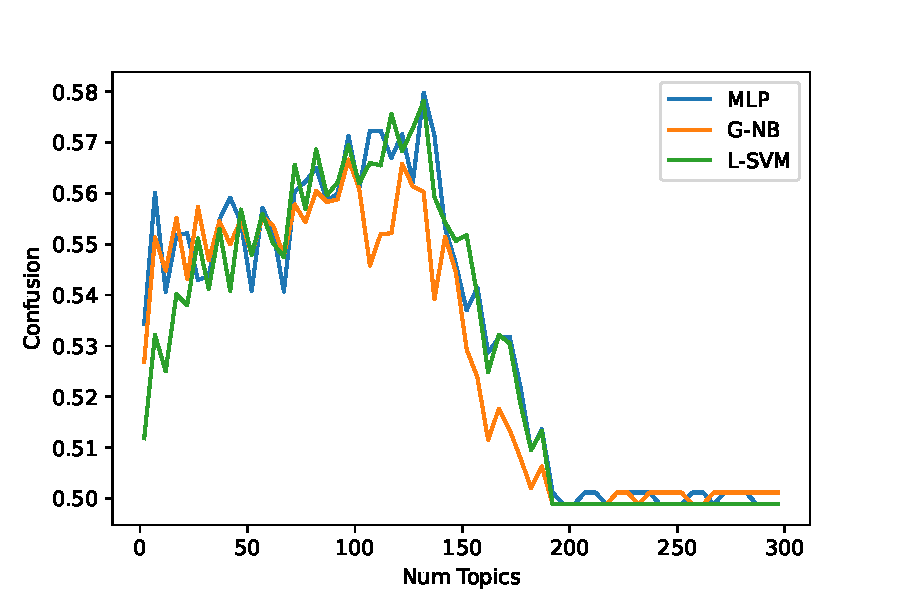
\includegraphics[width=.9\linewidth]{images/topic_confusion.pdf}
                \caption{Confusion over \# topics}
                \label{fig:conf}
            \end{figure}
        \end{column}
        \hspace*{-2cm}
       \begin{column}{.7\textwidth}
            \begin{figure}
                \centering
                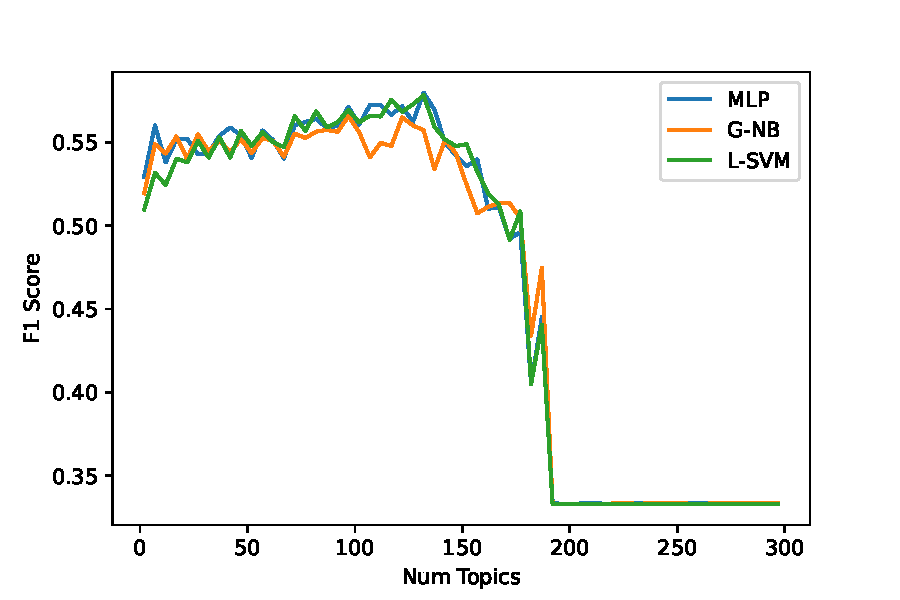
\includegraphics[width=.9\linewidth]{images/topic_fscore.pdf}
                \caption{F$_1$-Score over \# topics}
                \label{fig:f1}
            \end{figure}
        \end{column}
    \end{columns}
\end{frame}

\begin{frame}{LVM vs MLP vs G-NB (1)}
    \vspace*{-10mm}
    \begin{columns}
        \hspace{-5mm}
        \begin{column}{.7\textwidth}
            \begin{figure}
                \centering
                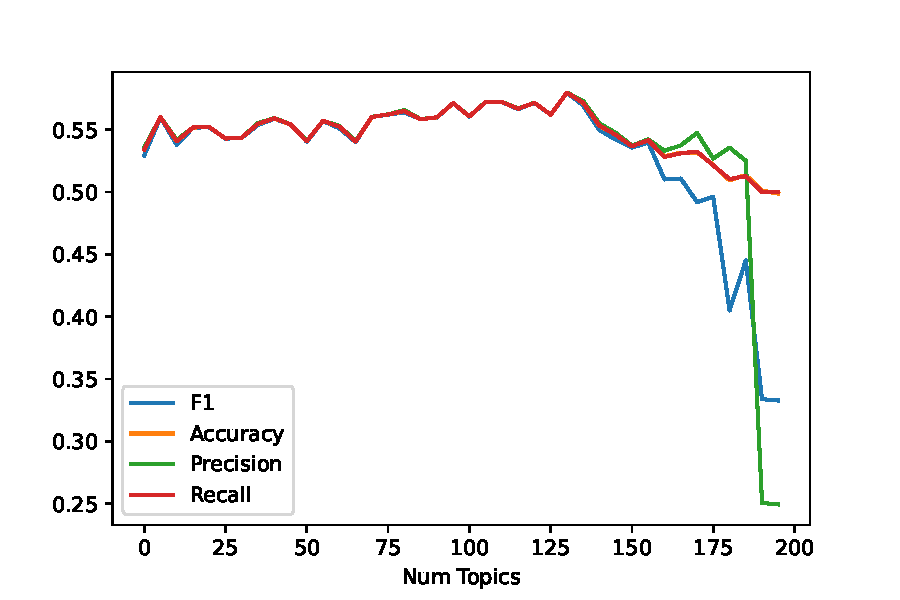
\includegraphics[width=.9\linewidth]{images/summary_mlp.pdf}
                \caption{MLP performance over \# topics}
                \label{fig:mlp}
            \end{figure}
        \end{column}
        \hspace*{-2cm}
       \begin{column}{.7\textwidth}
            \begin{figure}
                \centering
                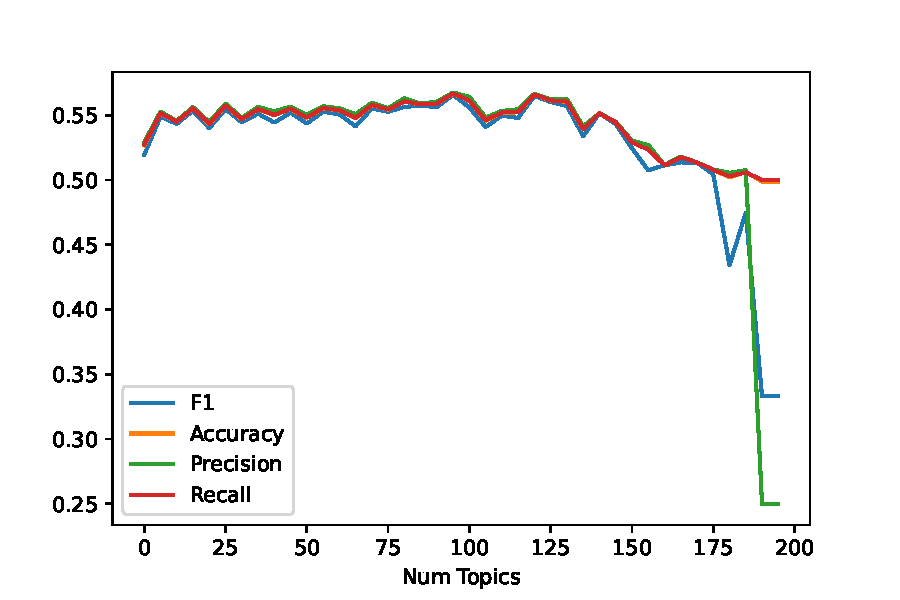
\includegraphics[width=.9\linewidth]{images/summary_g-nb.pdf}
                \caption{G-NB performance over \# topics}
                \label{fig:gnb}
            \end{figure}
        \end{column}
    \end{columns}
\end{frame}

\begin{frame}{LVM vs MLP vs G-NB (2)}
    \vspace*{-10mm}
    \begin{columns}
        \hspace{-5mm}
        \begin{column}{.7\textwidth}
            \vspace*{-10mm}
            \begin{figure}
                \centering
                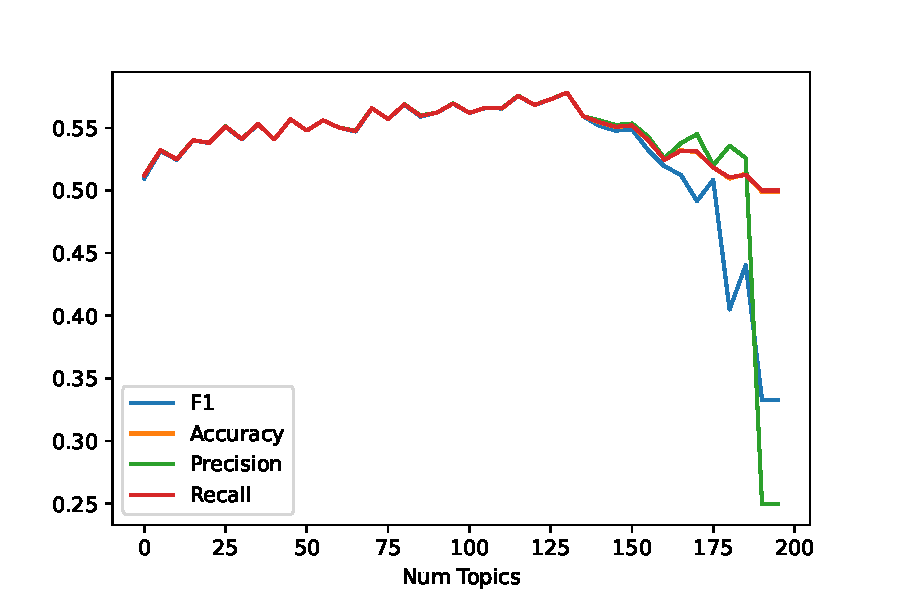
\includegraphics[width=.8\textwidth]{images/summary_l-svm.pdf}
                \vspace{-3mm}
                \caption{LVM performance over \# topics}
                \label{fig:lvm}
            \end{figure}
            \vspace{-7mm}
            
            \begin{columns}
                \begin{column}{.3\textwidth}
                     
                \end{column}
                \begin{column}{.7\textwidth}
                     {\footnotesize
                        \begin{itemize}
                            \item[Accuracy] 0.5651666666666667 
                            \item[Precision] 0.5651614499044595 
                            \item[Recall] 0.5651569102987339 
                            \item[F$_1$-Score] 0.5651535125604217 
                        \end{itemize}
                    }
                \end{column}
            \end{columns}
               
        \end{column}
        \hspace*{-2cm}
       \begin{column}{.7\textwidth}
            \begin{figure}
                \centering
                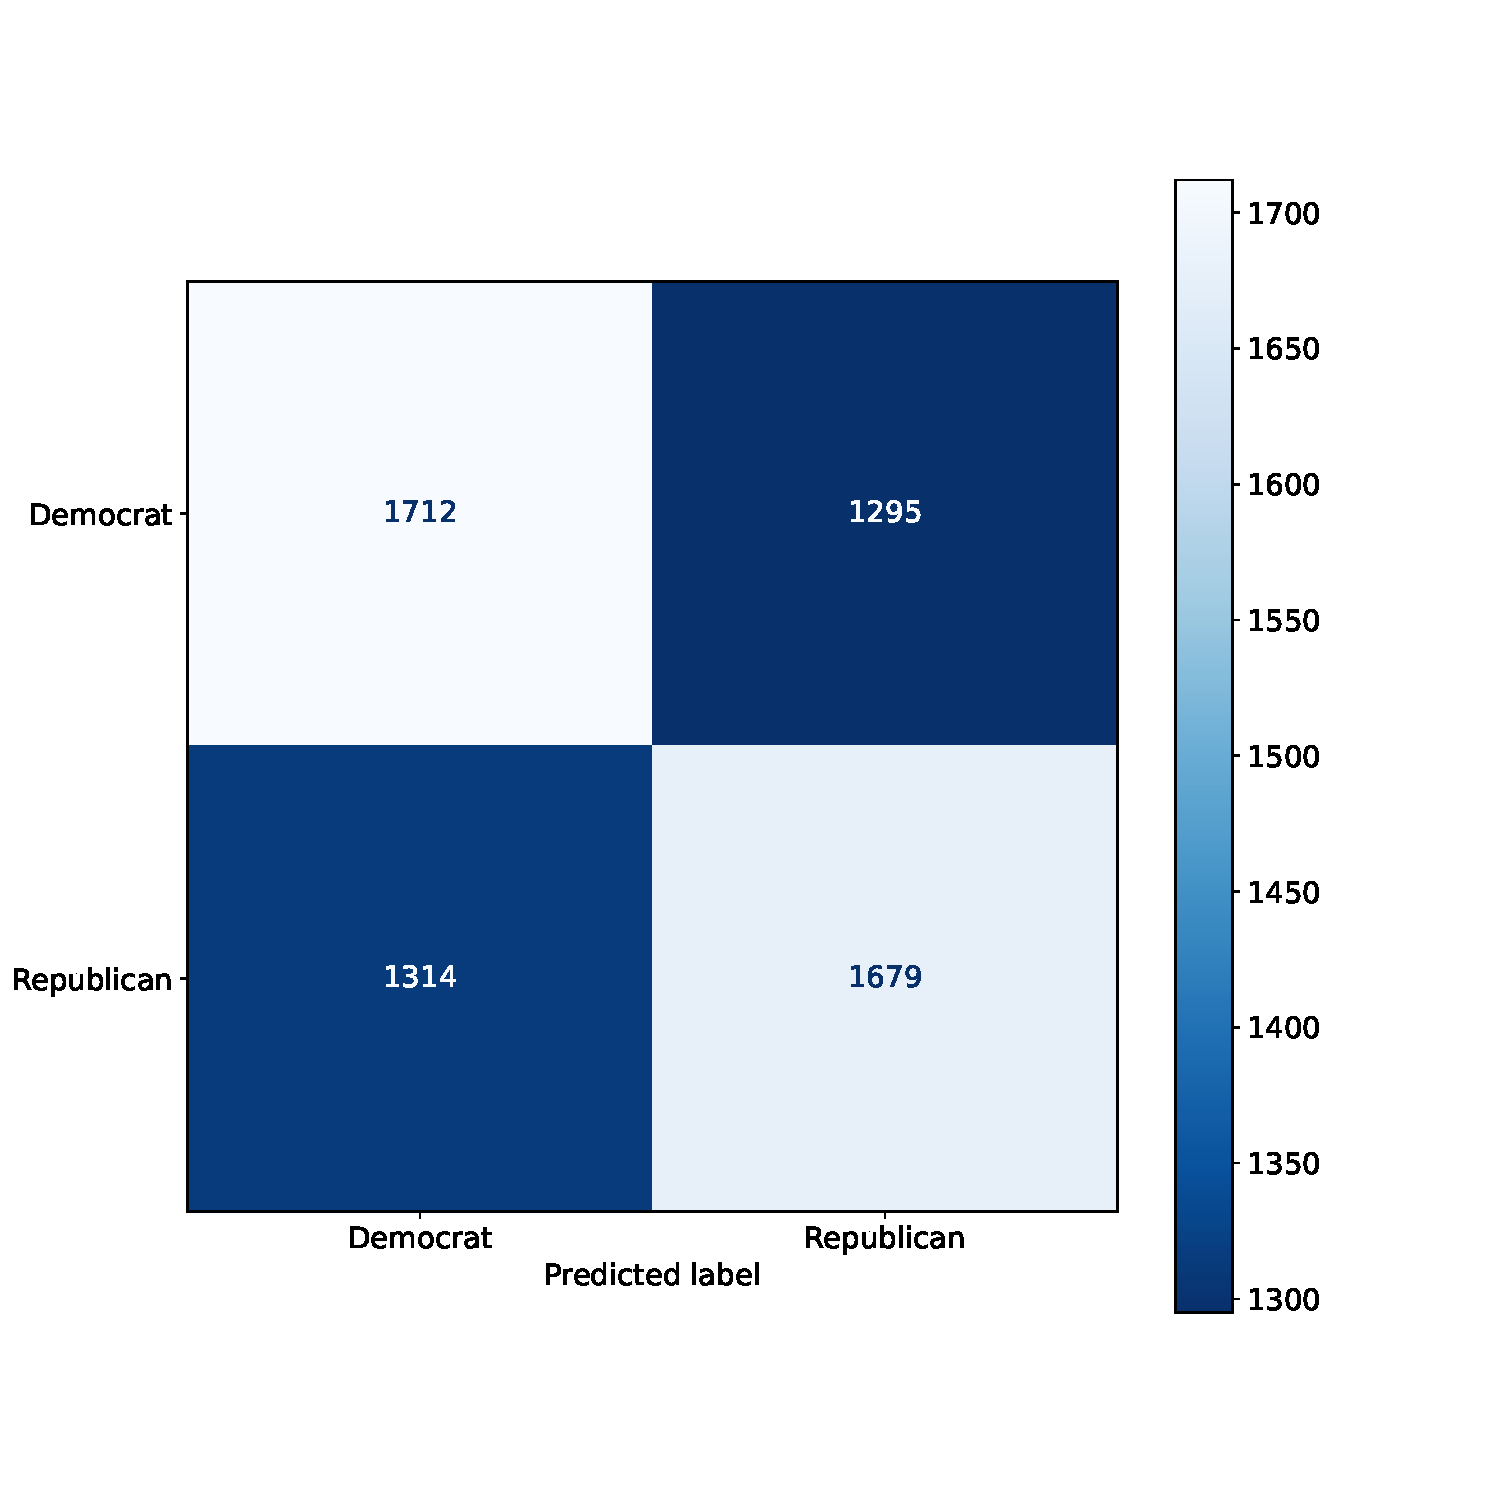
\includegraphics[width=.9\linewidth]{images/lvm_summary_130.pdf}
                %\caption{Confusion}
                \label{fig:lvm_summary_130}
            \end{figure}
        \end{column}
    \end{columns}

\end{frame}

\begin{frame}{Democrats vs Republicans}
    \vspace*{-5mm}
    \begin{columns}
        \hspace{-5mm}
        \begin{column}{.7\textwidth}
            \begin{figure}
                \centering
                
\includegraphics[width=.75\linewidth]{images/dem_wordcloud_full.png}
                \caption{Wordcloud Democrat}
                \label{fig:dem_wordcloud_full}
            \end{figure}
        \end{column}
        \hspace*{-2cm}
       \begin{column}{.7\textwidth}
            \begin{figure}
                \centering
                
\includegraphics[width=.75\linewidth]{images/rep_wordcloud_full.png}
                \caption{Wordcloud Republican}
                \label{fig:rep_wordcloud_full}
            \end{figure}
        \end{column}
    \end{columns}
\end{frame}

%------------------------------------------------
\section{Summary \& Outlook}
%------------------------------------------------

\begin{frame}{Summary \& Outlook}
    \vspace*{-5mm}
    \begin{columns}
        \hspace{-5mm}
        \begin{column}{.7\textwidth}
            \begin{figure}
                \centering
                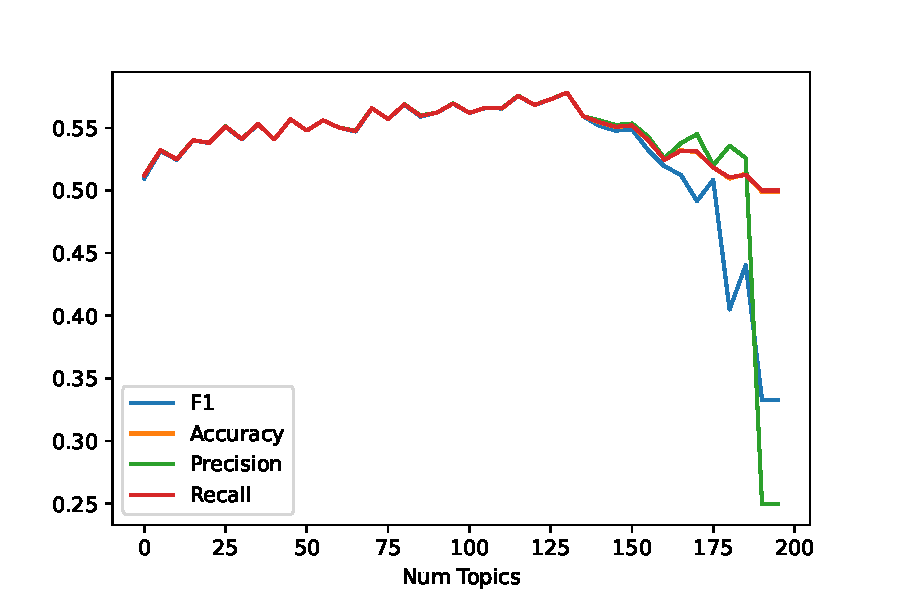
\includegraphics[width=.55\linewidth]{images/summary_l-svm.pdf}
                \label{fig:summary_lvm}
            \end{figure}
        \end{column}
        \hspace*{-4cm}
        \begin{column}{.7\textwidth}
            \begin{figure}
                \centering
                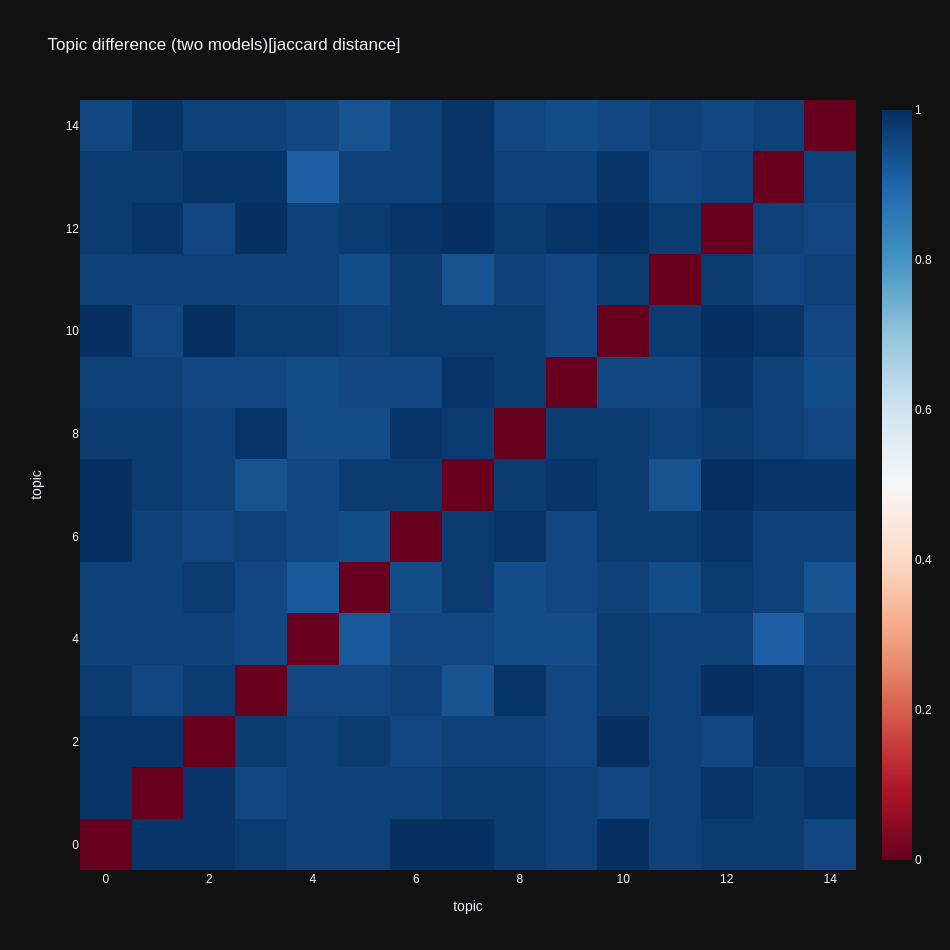
\includegraphics[width=.33\linewidth]{images/dem_dem_diff_15.png}
                \label{fig:summary_dem_rep_diff_15}
            \end{figure}
        \end{column}
    \end{columns}

    \begin{block}{Outlook}
        \begin{itemize}
            \item Refine pre-processing (modify TF-IDF or manually remove overlapping words)
            \item Adjust parameters of the LDA model and LVM classifier
        \end{itemize}
    \end{block}
    
    \begin{alertblock}{Result}
        \begin{itemize}
            \item First results do not look promising for reliable classification of posts.
        \end{itemize}
    \end{alertblock}

\end{frame}

%----------------------------------------------------------------------------------------

\end{document}
